\section{Results}\label{sec:results}

\subsection{Sigma Hyperparameter Selection}\label{subsec:sigmaHyperparameterSelectionResults}
Recall that $\sigma_1, \sigma_2, \ldots \sigma_n$ are hyperparameters that must be defined prior to executing the
algorithm.
The grid search exhausts every permutation $P_n^{\sigma_n}$, where:
\begin{equation}
    \label{eq:gridSearchQuerySigma}
    \sigma_n \ \in \ \{10^{-16}, 10^{-15}, \ldots 10^{1}\}
\end{equation}
% 2.22 * 10^-16 is the machine epsilon for double

\begin{figure*}
    \centering{
    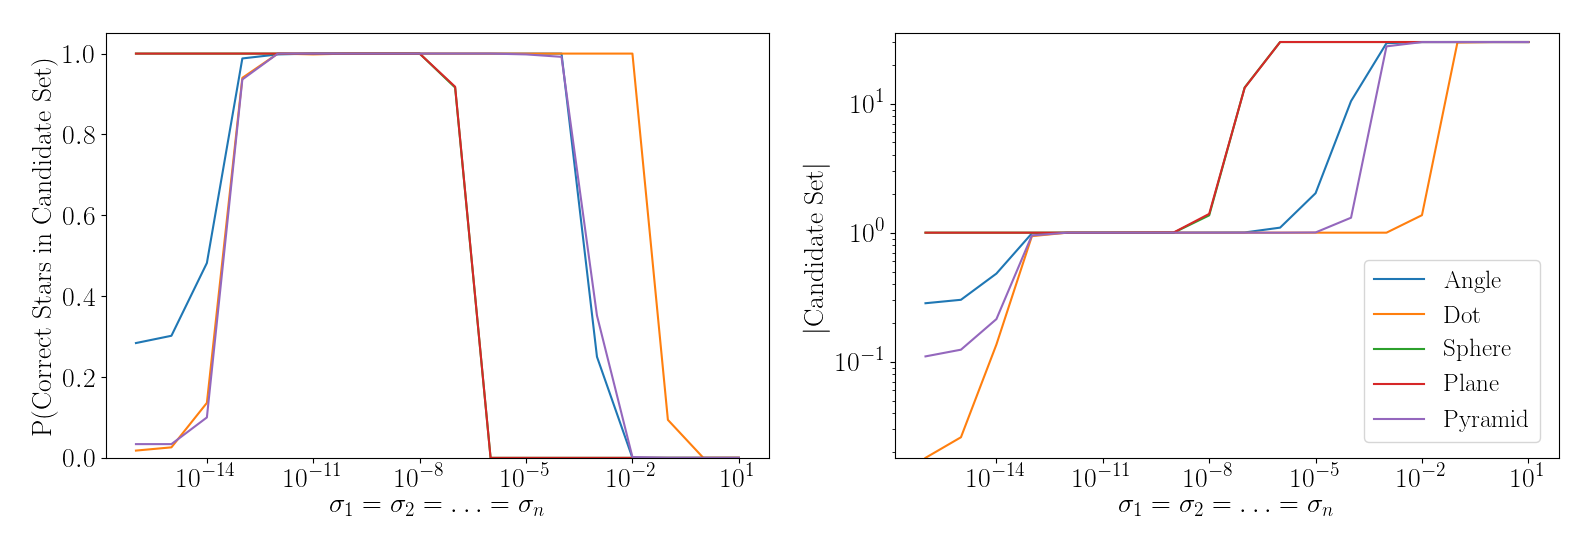
\includegraphics[scale=0.45]{images/sigma1-pcss-css.png}
    \caption{
    The left plot depicts the effect of varying $\sigma$ on the probability that the correct star set exists in the
    resulting candidates after the query.
    The right plot depicts the effect of varying $\sigma$ on the average size of the candidate set after the query, bounded
    by 30 candidates at maximum.
    The field-of-view is bounded by $f = 20^\circ$ and the apparent magnitude is bounded by $m = 6.0$.
    Each point represents the average of 1000 query steps without noise introduced.
    For brevity, all deviations associated with methods of more than one feature term (i.e.\ Dot Angle, Spherical
    Triangle, \ldots) had all corresponding $\sigma$ terms set equal to each other.
    } \label{figure:sigmaHyperparameterPlots}
    }
\end{figure*}

The set of plots in~\autoref{figure:sigmaHyperparameterPlots} depict the effect on different $\sigma$ terms against the
average size of the candidate set $S$ (on the left) and the probability that the correct stars exist in this candidate
set $Q$ (on the right).
If the deviation is too small, then the selectivity of each query becomes too restrictive and no results are returned.
On the other hand when the selectivity is too high, the candidate set size upper bound of 30 candidates is
hit and the chance that the correct candidate exists in the query declines.

The ideal period for all methods identifying images restricted by $f < 20 \land m < 6.0$ occurs when:
\begin{equation}
    \label{eq:idealRegionAcrossFeatures}
    \sigma_n \ \in (10^{-12}, 10^{-8})
\end{equation}
Regardless of the feature, a deviation choice between these bounds should be acceptable for distinguishing stars.

% Not including this, don't feel it is relevant to ideal analysis.
%It is important to note that each feature exists in different bounds.
%The values below represent the observed bounds of each feature:
%\begin{alignat*}{2}
%    \label{eq:observedFeatureSpace}
%    % Non-inclusive bounds given below.
%    \theta^{ij} &\in (2.6 \times 10^{-3} &&, 2.0 \times 10^1) \\
%    \theta^{ij} &\in  (2.6 \times 10^{-3} &&, 2.0 \times 10^1) \\
%    \theta^{ic}, \theta^{jc} &\in (2.6 \times 10^{-3} &&, 2.0 \times 10^1) \\
%    \phi &\in (1.3 \times 10^{-3} &&, 1.8 \times 10^2) \\
%    a^{ijk} &\in (3.1 \times 10^{-9} &&, 5.4 \times 10^{-2}) \\
%    \imath^{ijk} &\in (4.8 \times 10^{-16} &&, 5.3 \times 10^{-4}) \\
%    a^{ijk} &\in (3.7 \times 10^{-9} &&, 5.3 \times 10^{-2}) \\
%    \imath^{ijk} &\in (4.9 \times 10^{-16} &&, 5.3 \times 10^{-4})
%\end{alignat*}

% TODO: Replace these values with the ones using the most recent dataset.
\begin{table}
    \centering {
    \caption{
    Ideal query hyperparameter determination and sensitivity results of each method.
    The ideal region length $\ell$ represents the number of deviations where~\autoref{eq:idealQuery} is held.
    Each method's critical points $\sigma_{c1}$ and $\sigma_{c2}$ a is the upper bound on the $Q$ and $S$
    ideal region.
    } \label{tab:sensitivityIdealResults}
    \begin{tabular}{m{0.27\columnwidth}|m{0.13\columnwidth}|m{0.2\columnwidth}|m{0.2\columnwidth}}
        \textbf{Method} & $\ell$ & $\frac{\partial Q}{\partial\sigma} \text{ at } \sigma_{c1}$ &
        $\frac{\partial S}{\partial \sigma} \text{ at } \sigma_{c2}$ \\
        \hline \hline
        \textbf{Angle} & 3 & -0.375 & 0.001 \\ \hline
        \textbf{Dot Angle} & 9 & -0.453 & 0.183 \\ \hline
        \textbf{Spherical \newline Triangle} & 8 & -0.042 & 0.181\\ \hline
        \textbf{Planar \newline Triangle} & 6 & -0.041 & 0.001 \\ \hline
        \textbf{Pyramid} & 7 & -0.001 & 0.002
    \end{tabular}
    }
\end{table}

Referencing~\autoref{tab:sensitivityIdealResults}, there appears to some correlation between the number of
\textit{distinct} features and length of the stability region here.
The Dot Angle method uses three total features, two of which are distinct from each other ($\theta$ vs. $\phi$) for
it's query.
The Pyramid method uses three similar features, which has the same stable region length as the triangle methods
using two distinct features.
The Angle method uses only one feature for its query, and suffers in stable region length.

The candidate set size responses are most likely a result of the size of possible candidates that belong to each
method's respective feature (i.e.\ the number of rows of the table used in query).
The Angle method has the least number of possible candidates given the $f < 20 \land m < 6.0$ constraint, at 353700
possible catalog sets.
The triangle methods have roughly 35 times as many possible catalog sets as the Angle method.
The Dot Angle method has 3 times as many possible catalog sets as the triangle methods, and roughly 105 times as many
possible catalog sets as the Angle method.
Given a larger pool of results to choose from, it follows that the number of false positive increases as well.

The largest $Q$ response belongs to the Dot Angle method, while the smallest response belongs to the Pyramid method.
Unlike the candidate set size response, there appears to be no obvious correlation between the response of correct
star set existence and the number of features used.
If noise is not known, the most forgiving feature set in terms of both responses is the Pyramid method.

The $\sigma$ parameters for the following experiments were chosen using the results of the grid search, and selecting
the largest $\sigma_1, \sigma_2, \sigma_3$ (ordered as such) that maintained all the
conditions in~\autoref{eq:idealQuery}.
\begin{alignat*}{2}
    \text{Angle}&: \sigma_\theta &&= 10^{-4}\\
    \text{Pyramid}&: \sigma_\theta &&= 1.0 \times 10^{-4}\\
    \text{Dot Angle}&: \sigma_{\theta_{ic}} &&= 10^{-1}, \sigma_{\theta_{jc}} = 10^{-1}, \phi = 10^{-3} \\
    \text{Spherical Triangle}&: \sigma_a &&= 10^{-1}, \sigma_\imath = 10^{-11} \\
    \text{Planar Triangle}&: \sigma_a &&= 10^{-1}, \sigma_\imath = 10^{-11}
\end{alignat*}

In addition to the $\sigma_n$ parameters used in the previous experiments, a parameter $\sigma_o$ must be defined
prior to executing the \Call{FPO}{} method.
The linear search exhausts every overlay deviation selection:
\begin{equation}
    \label{eq:linearSearchSigmaOverlay}
    \sigma_n \ \in (10^{-16}, 10^{2})
\end{equation}

\begin{figure*}
    \centering{
    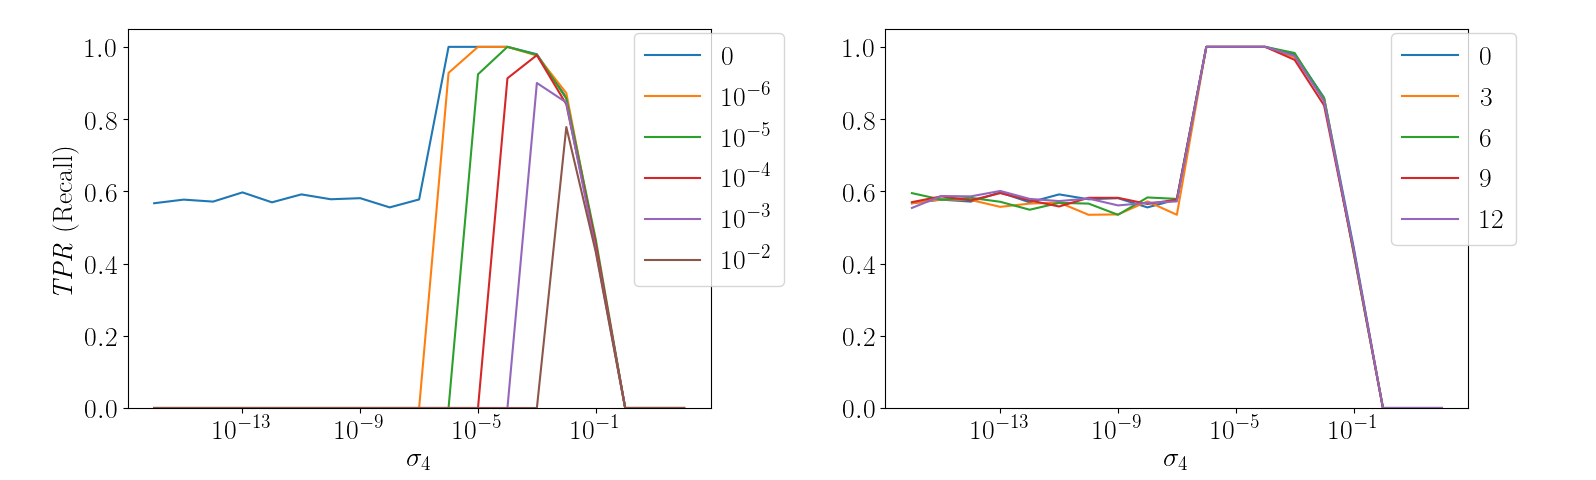
\includegraphics[scale=0.45]{images/sigma4-recall.png}
    \caption{
    Both plots depict the effect of varying $\sigma$ on the recall.
    The left plot depicts this relationship for different variations in noise, while the right plot depicts the same
    relationship for different numbers of false stars.
    The field-of-view is bounded by $f = 20^\circ$ and the apparent magnitude is bounded by $m = 6.0$.
    Each point represents the average of 200 query steps.
    } \label{figure:sigmaOverlayHyperparameterPlots}
    }
\end{figure*}

The set of plots in~\autoref{figure:sigmaOverlayHyperparameterPlots} depict the effect on different $\sigma$ terms
against the recall.
The period of accurate stability for Gaussian noise under $\sigma = 10^{-5}$ and for all false star introductions occurs
when:
\begin{equation}
    \label{eq:sigmaOverlayStableRegion}
    \sigma_4 \ \in (10^{-6}, 10^{-3})
\end{equation}

% TODO: Fix this here.
Looking at the both plots it is interesting to note that under no noise (Gaussian or false stars), a $\sigma_4 \ \in
(10^{-17}, 10^{-6})$ gives a recall of $~0.57 \pm 1.8 \times 10^{-2}$.
In this region, it appears that the \ldots
On the other end of the stability period for $\sigma_4 > 10^0$, accuracy drops straight to 0 regardless of the noise
presented.
At this period, stars are labeled with more weight to the order of the stars in the image rather than actually falling
within the specified deviation.

Focusing on the left plot of varying Gaussian noise, the accuracy dips to zero once the deviation of Gaussian noise
exceeds the selected deviation.
Past the $10^{-4}$ mark, the largest accuracy a deviation choice can achieve is no longer equal to one.
If noise is known, then the appropriate deviation for the \Call{FPO}{} method can be selected.
The right plot shows that the accuracy is not affected under different amounts of false stars.
Given varying amounts of false stars, virtually none of these stars were identified as an actual star.
The \Call{FPO}{} method is seen as highly specific, yielding no false positives.

The value of $\sigma_4 = 10^{-4}$ was selected for use in the \Call{FPO}{} method.
This is the largest deviation that lies in the accurate stable region.

\subsection{Query Selectivity}\label{subsec:querySelectivityResults}
Using the optimal hyperparameters described in the previous section, each query step was analyzed in terms of its
$Q$ and $S$ response to an introduction of Gaussian noise.

%\begin{figure*}
%    \centering{
%    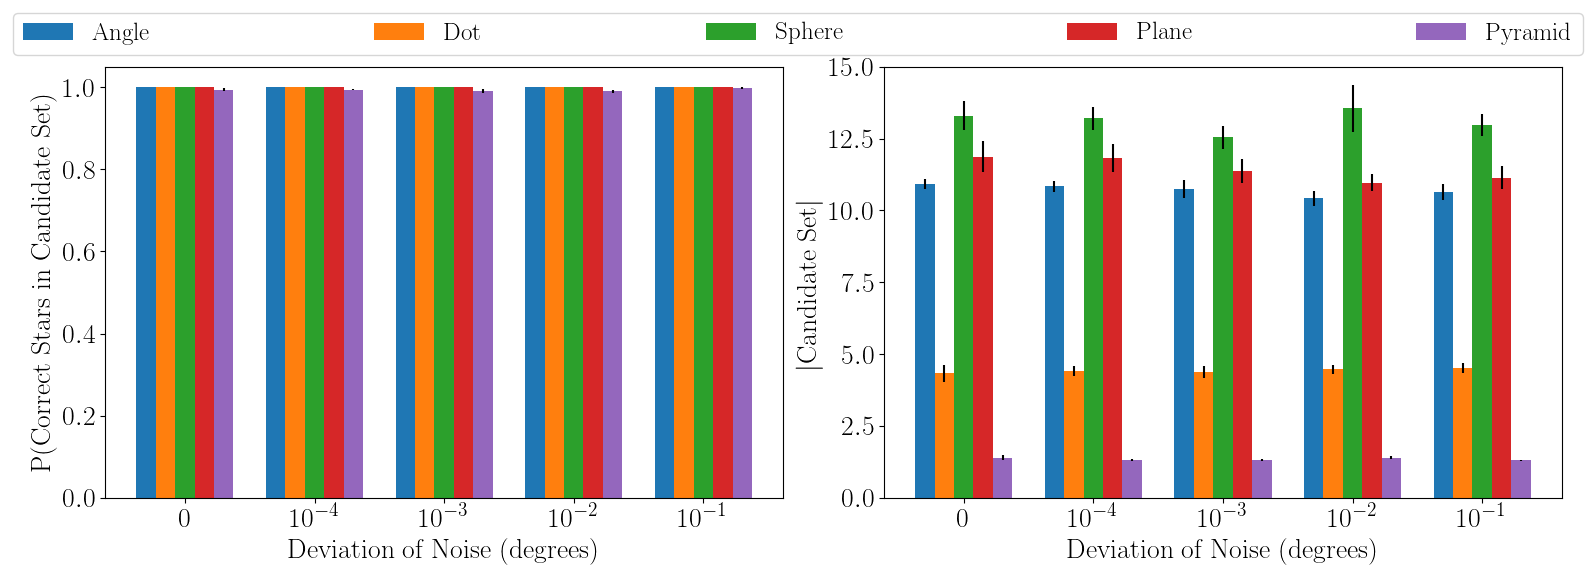
\includegraphics[scale=0.45]{images/query-exp.png}
%    \caption{
%    The left plot depicts the effect of varying the deviation of Gaussian noise on the probability that the correct
%    star set exists in the resulting candidates after the query.
%    The right plot depicts the effect of varying this same noise on the size of the candidate set after the query,
%    bounded by 5000 candidates at maximum.
%    Field of view limit is $f = 20^\circ$.
%    Each point represents the average of 5000 query steps.
%    For the probability measure these 5000 steps were split into 1000 averages, and the mean of these averages are
%    presented above.
%    } \label{figure:queryPlots}
%    }
%\end{figure*}

\begin{table}
    \centering {
    \caption{
    Each method's probability that the correct star set exists after querying ($Q$), average candidate set size ($S$),
    and query running time $t$ under no noise.
    Each point represents the average of 100 query steps.
    } \label{tab:queryExperimentResults}
    \begin{tabular}{m{0.18\columnwidth}|m{0.2\columnwidth}|m{0.2\columnwidth}|m{0.2\columnwidth}}
        \textbf{Method} & $Q$ & $S$ & $t \ (s)$  \\
        \hline \hline
        \textbf{Angle} & 1.00 & 10.63 & 00.25457 \\ \hline
        \textbf{Dot Angle} & 1.00 & 03.83 & 02.20369 \\ \hline
        \textbf{Spherical \newline Triangle} & 1.00 & 12.40 & 13.11543 \\ \hline
        \textbf{Planar \newline Triangle} & 1.00 & 12.44 & 12.34324 \\ \hline
        \textbf{Pyramid} & 0.98 & 01.72 & 00.35674
    \end{tabular}
    }
\end{table}

In~\autoref{tab:queryExperimentResults}, each method's $Q, S, \text{ and } t$ is displayed without the presence of
noise.
It is important to note that the data for the same experiment without the introduction of noise is very similar to that
with noise, suggesting that Gaussian noise does not affect the outcome of the query step.
Any inaccuracies with the overall identification process are most likely a result of future steps.

All methods are able to produce no false negatives after the query step except for the Pyramid method, whose accuracy
dips very slightly.
On the other hand, the Pyramid method consistently produces the smallest average candidate set size.
By sacrificing $Q$, the Pyramid method ensures a smaller average candidate set size.
This tradeoff can only be made when there exists other stars to choose from, as star trackers with a small number of
stars to choose from will be left without other combinations to identify stars from.

The next smallest average candidate set size can be seen with the Dot Angle method (4 candidates), followed by the
Angle method (11 candidates), and the triangle methods (12 for Spherical and Planar) last.
Feature sets involving angular separation are more selective than those using triangular features.

Recall that the Pyramid and Angle method use the same catalog, which is 35 times as small as the triangle method's
catalog.
This catalog size increases the query time for triangle methods by a factor of 100, meaning that roughly 100 Angle or
Pyramid queries cost the same as a single Spherical or Planar Triangle query.
It is interesting to note that the Dot Angle method has three times as many catalog entries for it's catalog, but is a
factor of 10 ms faster than the triangle methods.

Using the measure for efficiency in~\autoref{eq:queryEfficiency}, each method ranks as follows:
\begin{multicols}{2}
    \begin{enumerate}
        \item Pyramid
        \item Angle
        \item Dot Angle
        \item Planar Triangle
        \item Spherical Triangle
    \end{enumerate}
\end{multicols}

The Pyramid method has the most efficient query step.
The most efficient method that does not sacrifice accuracy is the Angle method.

\subsection{Candidate Reduction}\label{subsec:candidateReductionResults}
Using the same optimal hyperparameters described in~\autoref{subsec:sigmaHyperparameterSelectionResults}, each query +
reduction step was analyzed in terms of the average accuracy and efficiency response to Gaussian noise and false stars.

\begin{figure*}
    \centering{
    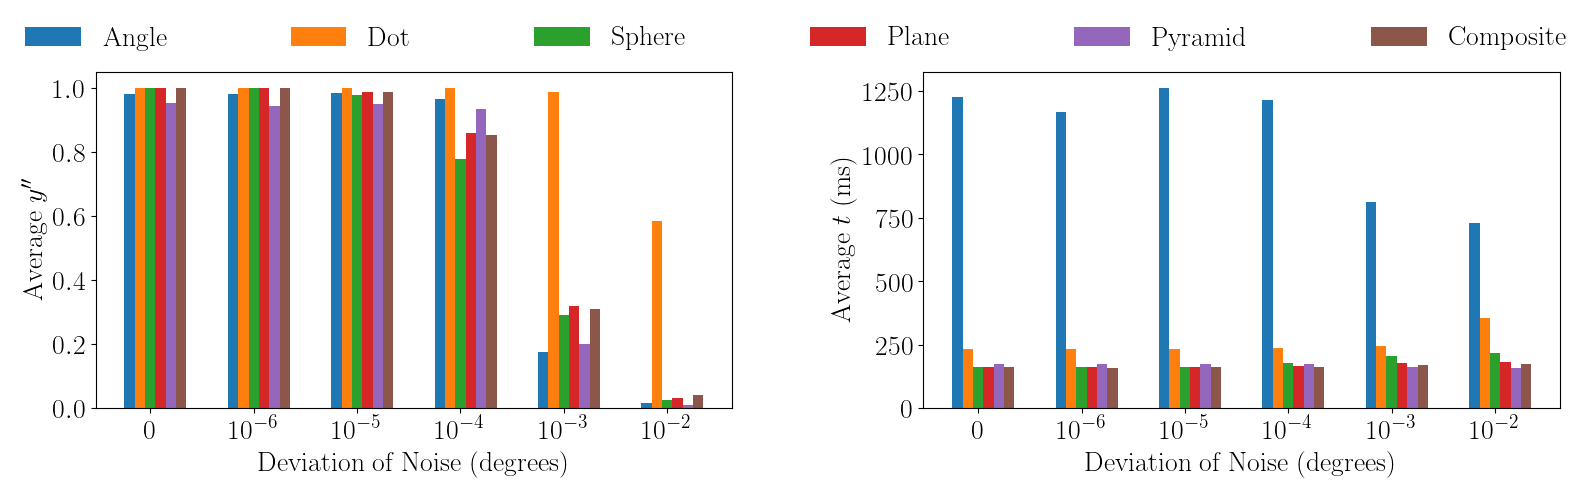
\includegraphics[scale=0.45]{images/reduction-shift-exp.png}
    \caption{
    Both plots depict the effect of varying the deviation of Gaussian noise on the average accuracy (left) and
    average running time to produce an $r$ set (right) for different identification methods.
    The field-of-view is bounded by $f = 20^\circ$ and the apparent magnitude is bounded by $m = 6.0$.
    Each method was capped at 100 query steps before erroring out and producing a false result.
    Each point represents the average of 100 reduction steps.
    } \label{figure:reductionShift}
    }
\end{figure*}

Without noise in both~\autoref{figure:reductionShift} and~\autoref{figure:reductionFalse}, only the triangle methods
had 100\% accuracy in reduction.
In terms of speed, the Pyramid method ranks first at an average of 210 ms per reduction run.
In terms of efficiency the Pyramid method ranks first again, with the largest accuracy to time ratio.
The tradeoff in accuracy for runtime appears to work in favor of the Pyramid method.

On the other end the Composite Pyramid is last in accuracy and last in runtime, using 293s on average to obtain an
accuracy of 64\%.
The Planar Triangle method uses the same features as the Composite Pyramid method, but runs 24 times as faster due to
its reduction step.
The $\{ R \mid 1 = |R| \}$ reduction step appears to be too aggressive of a filter and spends more time querying than
a pivoting reduction step.
The Spherical Triangle method runs twice as fast the Planar Triangle method, at an average time of 6.7s.
The Dot Angle method ranks below the Spherical Triangle but above the Planar Triangle method in terms of running time,
(9.2s) producing an average accuracy of 99\%.

In~\autoref{figure:reductionShift}, the deviation of Gaussian noise against the average accuracy and runtime is
displayed for different identification methods.
As soon as Gaussian noise of $10^{-5}$ degrees is introduced, all methods using triangular features drop to an average
accuracy of 42\%.
The rest of the methods experience a similar drop in accuracy (average of 18\%) for a Gaussian noise of $10^{-3}$
degrees.
The two main reasons for this later noise response are most likely the hyperparameters chosen, and the triangular
features themselves not being distinctive enough.

The hyperparameters for all methods were chosen without any noise introduced.
The upper bound of the ideal region for the angular separation feature was $\sigma_1 = 10^{-4}$.
It follows that any noise greater than this should lead to a decline in accuracy (average of 69\% decrease with
$\sigma = 10^{-3}$), which is seen in both the Pyramid and Angle methods.
The Dot Angle method decreases to 84\% given Gaussian noise of $10^{-4}$ degrees.
The query deviations for this method are greater than $10^{-4}$ degrees, but still show a similar response to the Angle
and Pyramid methods.

The Spherical / Planar Triangle methods have different reduction steps and features than the previous three methods,
and the response to noise occurs sooner than methods using angular features.
This may be due to the pivoting process, but a similar decline in the Composite Pyramid method (average of 54\%
decline with noise) argues that this may be a result of the triangular features themselves.
Increasing the accuracy here is possible by increasing $\sigma$, although~\autoref{tab:queryExperimentResults} shows
that triangular features already yield the highest number of candidates.
Increasing the deviation here would produce even more results, leading to a longer running reduction process.
What can be said here, is that the triangular features are highly sensitive to Gaussian error at the reduction step.

Looking at the running time plot on the right, an introduction of $10^{-5}$ degree noise to the Planar and
Spherical Triangle methods leads to an average increase of 141s per start to reduction step.
The Composite Pyramid method has a decline in running time as noise increases with a decrease of 293s at no noise, to
191s given noise of $10^{-2}$ degrees.
None of the other methods show a noticeable running time response to an introduction of Gaussian noise.

\begin{figure*}
    \centering{
    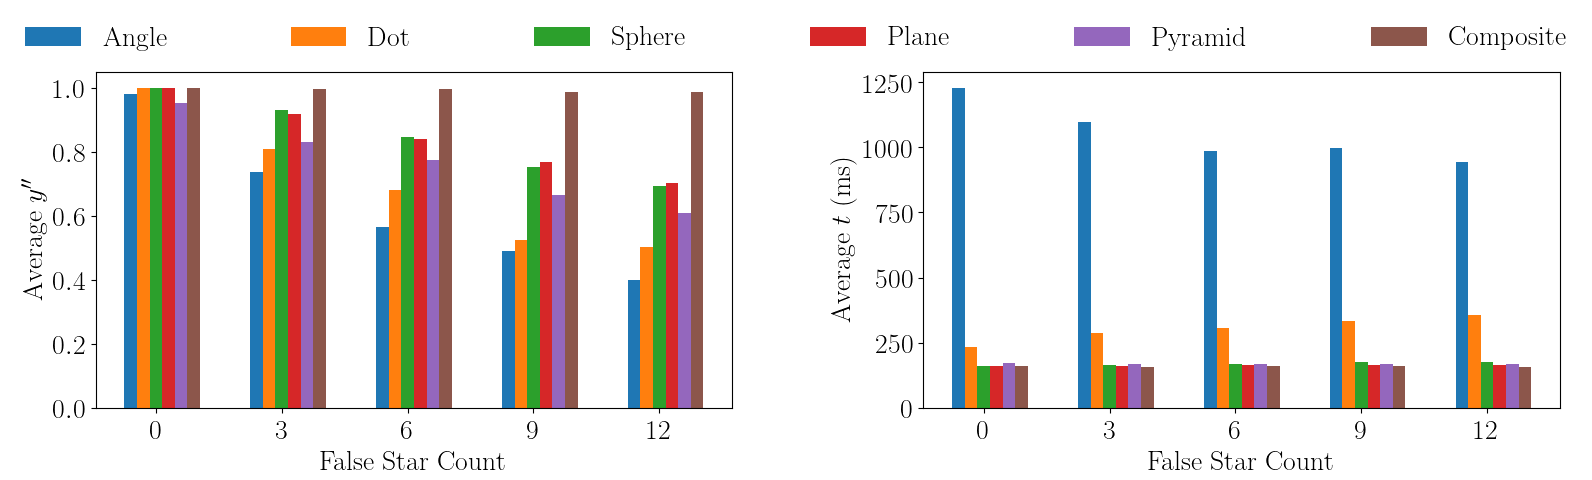
\includegraphics[scale=0.45]{images/reduction-false-exp.png}
    \caption{
    Both plots depict the effect of varying the number of false stars on the average accuracy (left) and
    average runtime to produce an $r$ set (right) for different identification methods.
    The field-of-view is bounded by $f = 20^\circ$ and the apparent magnitude is bounded by $m = 6.0$.
    Each method was capped at 100 query steps before erroring out and producing a false result.
    Each point represents the average of 100 reduction steps.
    } \label{figure:reductionFalse}
    }
\end{figure*}

In~\autoref{figure:reductionFalse}, the number of false stars against the average accuracy and runtime is displayed
for different identification methods.
It is easier to observe a trend in the noise here.
The number of false stars is generally proportional to the number of query steps, and inversely proportional
to the accuracy.
The general rank of the accuracy of all methods as the number of false stars increases is listed below:
\begin{multicols}{2}
\begin{enumerate}
    \item Pyramid
    \item Planar Triangle
    \item Spherical Triangle
    \item Dot Angle
    \item Angle
    \item Composite Pyramid
\end{enumerate}
\end{multicols}

In 1st place is the Pyramid method, which has the best accuracy (63\%) given an image with 12 false stars.
The Pyramid method specifies a false star persistence avoidance process for choosing query star sets from the image, and
the effectiveness of this can be seen.
The Composite Pyramid uses the same false star persistence avoidance method, but the difference in features render this
technique less effective than all other identification methods (21\% at 12 false stars).
The Spherical and Planar Triangle methods show that the pivoting process is fairly effective in handling false stars,
with an average accuracy of 35\% and 45\% respectively.

The Dot Angle method and the Angle method rely purely on the $|R| = 1$ reduction filter, which handles false stars less
effectively than pivoting or choosing query steps differently.
The Dot Angle and the Angle method have an average accuracy of 39\% and 30\% respectively at 12 false stars.

The Pyramid method's false star persistence avoidance process works best for handling the false stars, but the
pivoting process works fairly well too.
Both of these are perform at different steps in the general identification flow, and it may be interesting to combine
the two, use different query features, and see if it handles false stars even better.

Under both types of noise with the current approaches listed here, the best average accuracy to efficiency ratio
belongs to the Pyramid method.

\subsection{Identification Determination}\label{subsec:identificationDeterminationResults}
Using all optimal hyperparameters described in~\autoref{subsec:sigmaHyperparameterSelectionResults}, each identification
was ran end-to-end and analyzed in terms of its response to an introduction of Gaussian noise and false stars.

\begin{figure*}
    \centering{
    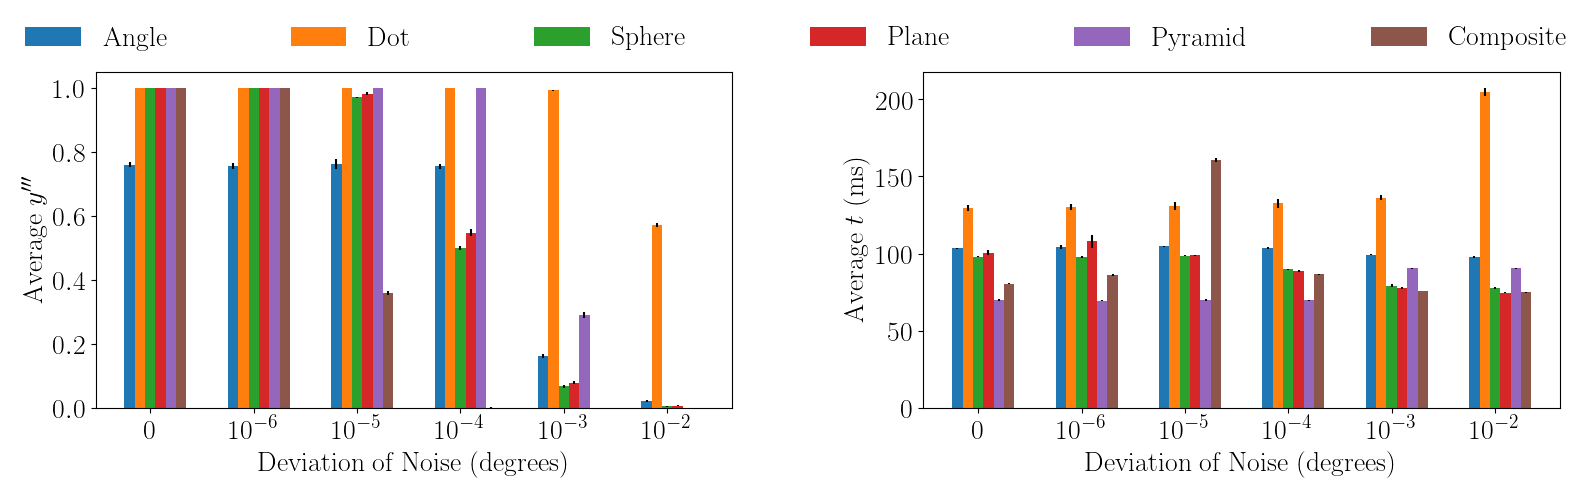
\includegraphics[scale=0.45]{images/identification-shift-exp.png}
    \caption{
    Both plots depict the effect of varying the deviation of noise on the average accuracy (left) and average
    running time to produce a map $a$ (right) for different identification methods.
    The field-of-view is bounded by $f = 20^\circ$ and the apparent magnitude is bounded by $m = 6.0$.
    Each method was capped at 100 query steps before erroring out and producing a false result.
    Each point represents the average of 100 identification steps.
    } \label{figure:identificationShift}
    }
\end{figure*}

Without noise in both~\autoref{figure:identificationShift} and~\autoref{figure:identificationFalse}, all methods except
for the Angle and Composite Pyramid yield 100\% accuracy.
Out of these 100\% accuracy methods, the Pyramid method had the shortest running time here, running an average of
214ms to obtain a result.
The Dot Angle method is 2nd in this group, requiring 8.5s to obtain a result.
The Spherical and Planar Triangle methods follow here, running an average of 14.2s to obtain a correct result.
Out of the two methods that are not 100\% accurate under no noise (Angle, Composite Pyramid), the Angle ran the fastest.
The Composite Pyramid took the longest to run, at 324s to obtain a result.

Comparing the results found in reduction experiment without noise to these results here, the Pyramid and Dot Angle
methods rely on the~\autoref{figure:genericIdentificationMethodFlowchart} filter after the reduction step to boost
its accuracy to 100\%.
The Angle method shows no difference in accuracy here, but the Composite Pyramid method appears to decline from 64\%
to 44\%.
Given that all triangle methods use the \Call{DMT}{} call in its identification step, the culprit here appears to be
from the \Call{VerifyC}{} procedure.
This may be another strong filter that is hindering the performance of the Composite Pyramid method, similar to its
reduction step.

In~\autoref{figure:identificationShift}, the deviation of Gaussian noise is displayed against the average accuracy and
running time.
When noise of $10^{-5}$ degrees is introduced, the same decline in accuracy as seen in the reduction experiment can be
seen here.
All methods using triangular features decline to an average accuracy of 31\%.
The identification step of all triangular feature methods involve the \Call{DMT}{} procedure.
Inaccuracies in this procedure can be found by subtracting the accuracies found in the reduction
experiment by those found here.
This average difference is 10\%, suggesting that the \Call{DMT}{} call does account for some of the additional
inaccuracy.

When noise of $10^{-3}$ degrees is introduced, all methods with angular features decline to an average accuracy of
18\%.
This is where all angular methods sharply dropped in accuracy for the reduction experiment, and it follows that the
accuracy in the previous steps should affect the future steps (identification).
For the Angle method, the \Call{DMT}{} call is another limiting factor for accuracy.
Recall that the $\sigma$ value chosen for the \Call{FPO}{} procedure was $10^{-4}$.
Any differences beyond the overlay $\sigma$ will not be counted, and the \Call{DMT}{} call will have less
information to work with.

The Dot Angle method shows no difference between its reduction accuracy and identification accuracy.
This method determines the $a$ map at query time, and it follows that no additional inaccuracies can occur after
reduction.
The Pyramid method has a higher accuracy than its reduction results, showing that the \textit{Confident in $r$?} filter
is fairly effective.
This method is the most accurate and quickest under the most noise ($10^{-3}$ degrees), requiring roughly 193ms to
run from start to finish.

The only methods that appear to have a significant running time response to noise are those with triangular features.
Given that these methods have the most expensive query (at 12.7s per query), any additional queries will be penalized.
The average increase in running time for the Spherical and Planar Triangle methods with images of no noise to those with
$10^{-3}$ degrees of noise is 216s.
For the Composite Pyramid, there appears to be decrease in running time as the noise increases (decrease of 90s from
no noise to $10^{-3}$ degrees of Gaussian noise).
The Angle method is the 2nd fastest identification method (285ms), followed by the Dot Angle method (7.7s).

%When noise of $10^{-6}$ degrees is introduced, all methods decline XXX\% on average in accuracy.
%Previously in the reduction experiment, accuracy declined near to zero for the Spherical and Planar Triangle methods.
%Low accuracy there, but accuracy on-par here shows a strong $r$ confidence decision step for these methods.
%On the other end, the Composite Pyramid always iterates to the $\tau = 100$ limit beyond this, showing that the
%candidate reduction step for this method is not able to produce a confident result in a reasonable amount of time.
%
%When noise of $10^{-5}$ degrees is introduced, all methods decline further to an average of XXX\% accuracy.
%It is important to mention that although this contrasts the accuracy stability seen with increasing Gaussian noise
%in the reduction experiment, error could still stem from the reduction stage.
%The $y''$ measure for the reduction experiment only records whether the returned $r$ set exists in the original,
%non-rotated image set.
%This does not mean that this returned catalog set correctly matches with the current query star set.
%
%This problem does not seem to stem from the \Call{FPO}{} procedure,
%as~\autoref{figure:sigmaOverlayHyperparameterPlots} shows that the classifier effectiveness declines around
%$10^{-4}$ for the deviation we are currently using.
%Instead, the \Call{DMT}{} procedure that uses the overlaying procedure may the source of error.
%As input to \Call{FPO}{}, we require two sets of stars \textit{and} a rotation.
%This rotation is heavily dependent on the current location of stars in both the image and the catalog.
%Because the stars in the image have been shifted, the given rotation is wrong and the returned $M$ sets will most likely
%yield no matches.
%
%As \Call{DMT}{} exists now, a map will arbitrarily chosen if all $M$ sets are empty.
%An extra verification step might be useful in \Call{DMT}{}, to prevent choosing a map at chance.
%If noise is known in advance, then increasing the overlay $\sigma$ would also prevent this from negatively impacting
%accuracy.

%Additional inaccuracies may also stem from the \Call{VerifyP}{} and \Call{VerifyC}{} steps in the Pyramid
%and Composite Pyramid methods.
%These are additional verification steps required before returning a map.
%These procedures may be too exclusive, skipping potential true positives
%Recall that the Pyramid and Composite Pyramid methods include a verification step before returning the map.
%The \Call{VerifyP}{} and \Call{VerifyC}{} may be too exclusive, skipping potential true positives.
%Removing this step may yield better accuracy for both methods.

In~\autoref{figure:identificationFalse}, the number of false stars against the average accuracy and runtime is
displayed for different identification methods.
In 1st place again, with close to 100\% accuracy given any number of false stars is the Pyramid method.
The effectiveness of the false star persistence avoidance process combined with the \textit{Confident in $r$?} filter
shines here.
This same false star persistence avoidance process might also attribute to the Composite Pyramid not declining in
accuracy as much as the other methods (but it still does decline).

All other methods (Spherical / Planar Triangle, Angle, Dot Angle) appear to decline to the same accuracy at 35\%
given 12 false stars, indicating that choosing query steps is vital in properly handling false stars.
For all of these methods a false star is for the outer loop means iterating through every combination of stars with
this false star.
Any result that is returned from here to the next iteration of the outer loop will be false, and it is important to
cycle through as many unique image star sets as possible to avoid this problem.

As the number of false stars increases, the running time increases for the Spherical and Planar triangle methods.
For each three false star increment, there is an average of 40s increase in running time.

For the other methods, there does not appear to be a response to running time here as the number of false stars
increases.
In order of shortest running time, each method ranks as follows:
\begin{multicols}{2}
    \begin{enumerate}
        \item Pyramid
        \item Angle
        \item Dot Angle
        \item Planar Triangle
        \item Spherical Triangle
        \item Composite Pyramid
    \end{enumerate}
\end{multicols}

The Pyramid method is ~1500 as fast as the Composite Pyramid method, requiring an average of 211ms to present a result
given an image of 12 false stars.
The Angle method is a close 2nd place, with an average running time of 240ms.
Distant from 2nd place and 4th is the Dot Angle method, with an average running time of 6.7s.
The Spherical and Planar Triangle methods require an average of 107s to produce a result.

The Pyramid method is the best identification method for handling images with both types of noise, and is also the
most efficient.

\begin{figure*}
    \centering{
    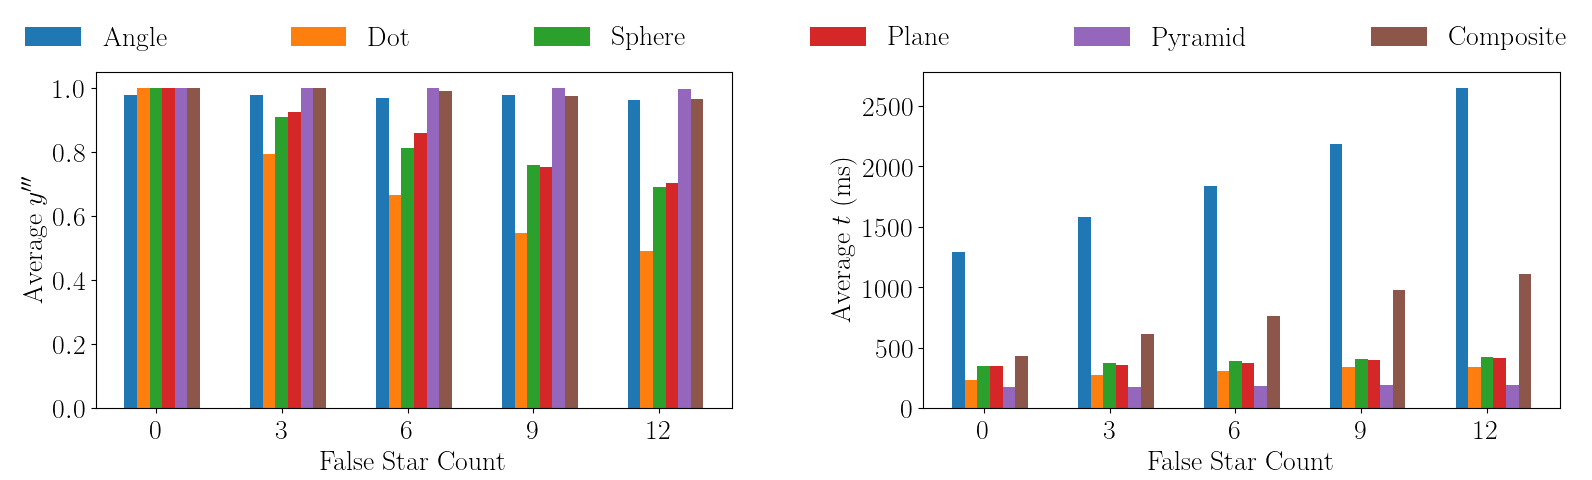
\includegraphics[scale=0.45]{images/identification-false-exp.png}
    \caption{
    Both plots depict the effect of varying the number of false stars on the average accuracy (left) and average running
    time to produce a map $a$ (right) for different identification methods.
    The field-of-view is bounded by $f = 20^\circ$ and the apparent magnitude is bounded by $m = 6.0$.
    Each method was capped at 100 query steps before erroring out and producing a false result.
    Each point represents the average of 100 identification steps.
    } \label{figure:identificationFalse}
    }
\end{figure*}
